\chapter{Introduzione ai sistemi automatici di misura}
Nel seguente esempio si riporta come viene effettuato il collaudo di un filtro
passa-basso, si organizza il comparto di misura disponendo un generatore di
segnale opportunamente configurato, il DUT (Device Under Test) e uno strumento
di misura.

Per effettuare il collaudo del filtro va organizzato il banco di misura
prendendo un generatore di
segnale (sorgente)
applicando uno stimolo di tipo sinusoidale e usando successivamente un
oscilloscopio o un multimetro
per misurare la grandezza
in ingresso e quella in uscita.

Effettuando la misura dei due valori e calcolato il guadagno è poi possibile
riportare i valori su
un grafico e realizzare la maschera del filtro, la prova va effettuata con più
valori di frequenza.

Considerando una n-pla di frequenze con n sufficientemente grande si può
ripetere il test
rispettando una ovvia semantica, configurando prima la sorgente, attendendo un
tempo di
assestamento, poi effettuando le misure con il sistema a regime stabile.

Il tecnico coordina l'attività degli strumenti attivando la sorgente al tempo
giusto e attiva
l'intervento del multimetro quando è necessario l'intervento del multimetro,
eseguendo il test in
maniera ordinata da frequenze più basse a più alte o viceversa, sarebbe invece
curiosa una scelta
disordinata delle frequenze, nonostante talvolta abbia senso farlo, ad esempio
su dispositivi con
comportamento "isteretico".

\begin{figure}[h]
\centering
\begin{circuitikz}[]
\draw
 (0,0) to [short , *-] ++(1,0)
        to [R,l=R] ++(2,0)
        to [C,l=C] ++(0,-2) to [short,-*] ++(-3,0);
\draw (0,-2) to [open,v^>=$v_{in}$] ++(0,2);
\draw (3,-2) to [short,*-*] ++(1,0)
             to [open,v=$v_{out}$] ++(0,2)
             to [short, *-*] ++(-1,0);
\end{circuitikz}
\caption{Filtro passa-basso}
\end{figure}

Nell'analisi di un filtro è anche importante studiarne la \textit{fase},
potrebbe essere
presente anche una maschera della risposta in fase richiesta dal committente,
ovvero lo sfasamento
prodotto dal DUT alle basse frequenze; si ritiene che le deviazioni siano
contenute se i punti vicini in
frequenza sono vicini tra loro in fase.

Per misurare lo sfasamento tra segnali isofrequenziali, è possibile usare
un oscilloscopio
oppure strumenti dedicati come i contatori universali, utilizzando il contatore
"counter" a due
canali si può misurare il ritardo di fase dell'uscita rispetto all'ingresso.
%AGGIUNGI IMMAGINE SFAASAMENTO
\begin{figure}[h]
\centering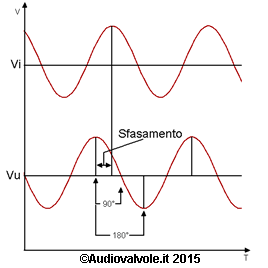
\includegraphics[width=0.4\linewidth,trim={0 4mm 0
0},clip]{misurasfasamento}
\caption{$\Delta\varphi = 2\pi \frac{\tau}{T_0}$}
\end{figure}


\subsection{Ruolo dell'operatore}
Questo ruolo può essere demandato per realizzare il processo in modo automatico,
in questo caso l'operatore
svolge il processo di coordinamento tra le sorgenti, analizzando i risultati dei
vari strumenti per
elaborare i risultati e annotarli in un diagramma.

Queste azioni possono essere demandate ad un'unità funzionale (UF) che svolge il
lavoro
dell'operatore, quest'unità è spesso un calcolatore, si possono attivare infatti
le funzioni degli
strumenti colloquiando attraverso questi tramite un'opportuna interfaccia
digitale, ovvero uno
strumento elettronico-digitale può essere configurato senza alcuna azione fisica
sul suo front
panel ma può essere configurato tramite la sua interfaccia, ovvero inviando allo
strumento una
sequenza di caratteri, una stringa, che viene decodificata e interpretata
dall'interfaccia dello
strumento, ad esempio:

Stringa per generare una forma d'onda sinusoidale di 10 V picco-picco, 1000 Hz
e un offset DC di 0 V:

\noindent
\verb|APPLY:SINusoidal 10, 1000, 0|

Quest'operazione si poteva fare a partire dagli anni 70, si realizzarono dunque
le prime stazioni
automatiche di misura.
L'unità funzionale è una macchina che può essere programmata, solitamente un PC,
era collegata ai
vari strumenti attraverso un BUS, deve poter inviare e ricevere messaggi e
informazioni ai vari
strumenti di misura.

Le spinte per cui si andò a studiare e applicare soluzioni di questo genere
erano legate ad
esigenze di incrementare l'affidabilità e velocizzare i processi di misura e
ridurne i costi.

Il collaudo affidato ad un tecnico richiede un certo tempo (del tecnico), se si
effettua produzione
di massa di dispositivi questa operazione manuale è impensabile, si effettua
inizialmente un
collaudo campionario, non si collauda ogni singolo campione ma deve comunque
essere una popolazione
rappresentativa, se anche si producono un milione di pezzi almeno un centinaio
andrà
collaudato, quanto tempo ci vorrebbe con un operatore umano? I tempi sarebbero
troppo lunghi,
l'affidabilità del collaudo è inoltre scarsa essendo affidata a all'operatore
umano, nella prima
ora ad esempio il tecnico lavora bene, nelle successive sarà sempre più stanco
\textit{lanciando i filtri
passa-basso dalla finestra}, il costo umano per le risorse umane inoltre è
elevato.

Se si programma un PC con tutte le istruzioni, la configurazione dello
strumento di misura, oscilloscopio a due canali, sarà del tipo

\begin{verbatim}
MEAS:CH1:VAC?
MEAS:CH2:VAC?
\end{verbatim}

queste istruzioni possono essere inserite in una struttura ciclica per ogni
valore di frequenza. Ne guadagno in affidabilità, un macchina programmata
quando esegue una struttura ciclica, non si stanca nella riproduzione
ripetitiva delle stesse azioni, la macchina non fa altro di ciò che è
codificato nelle istruzioni.
Se ne guadagna anche nel tempo di interazione per
configurare la sorgente ad esempio che va a regime in tempi inferiori a quelli
necessari all'operatore a cambiare le impostazioni, invece mediante
l'interfaccia le istruzioni e le risposte ottenute hanno ordini di grandezza di
gran lunga inferiori, lo stesso intero collaudo sulle varie frequenze può essere
eseguito in frazioni di secondi.

Di contro il controller non è in grado di interagire in caso di eventi
imprevisti se questi non
sono appunto "previsti" e configurate le rispettive risposte dell'unità di
controllo.
L'operatore dovrebbe trasferire tutta la sua conoscenza nella macchina,
aggiungendo inoltre
ulteriori sensori alla stazione di misura, magari non direttamente collegati al
fenomeno.

Sostenuto l'investimento iniziale della programmazione dell' UF non è più
necessaria una squadra di
tecnici al fine di collaudare tutti i DUT, è necessario solo un tecnico (o una
macchina) che
posizioni e selezioni gli oggetti che superano il test o meno.

\section{Interfaccia standard IEEE 488 - GPIB}
La seguente interfaccia è ritenuta uno standard dagli anni 70, GPIB sta per
\textit{General Purpose Interface Bus} sviluppata da HP, successivamente il
ramo riferito agli strumenti di misura è diventato Agilent e poi KeySight.

Inizialmente l'interfaccia si chiamava HPIB, gli altri costruttori poi
standardizzarono le specifiche dell'interfaccia per complementare i loro
strumenti di misura con quest'interfaccia, presentano un certo connettore con
una porta standard.
\begin{figure}[h]
\centering
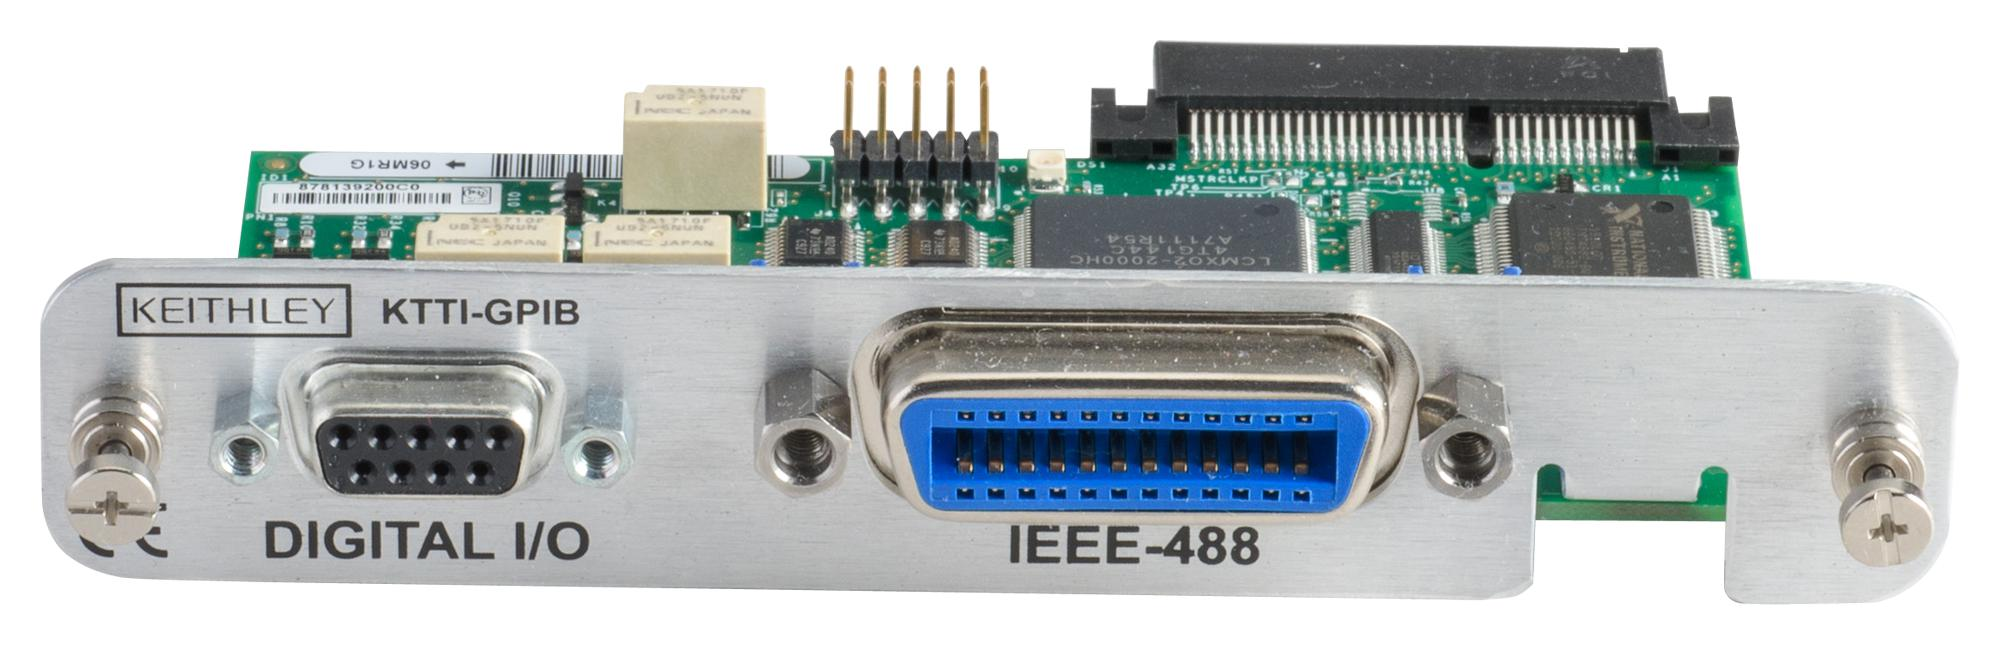
\includegraphics[width=0.9\linewidth]{GPIB}
\caption{Periferica GPIB con rispettiva porta (in blu)}
\end{figure}

Il PC potrebbe non essere disposto dell'interfaccia GPIB, si potrebbe
aggiungere una scheda PCI per avere le funzionalità della porta GPIB, oggi si
preferisce utilizzare delle versioni miniaturizzate GPIB-USB rendendo il
collegamento dell'interfaccia più semplice.

Per realizzare il collegamento si utilizza un connettore standard della
lunghezza solita di 2 m con dei connettori ``ermafroditi'' rendendo possibile
impilare i connettori nello stesso punto.

La topologia del BUS non è classificabile né di tipo a ``stella'' con un nodo
principale, né c'è un BUS ad anello chiuso (daisy chain), si possono realizzare
topologie ibride per raggiungere ed interconnettere tutte le unità tra loro, il
BUS contiene 25 linee, ogni linea verrà forzata ad un certo potenziale
elettrico, questo verrà condiviso tra tutti i dispositivi collegati al BUS, a
causa del collegamento elettrico franco, il potenziale sarà lo stesso.

Lo standard fornisce le specifiche elettriche, meccaniche e funzionali.
Le linee attive all'interno del BUS sono in realtà 24, la venticinquesima è
inutilizzata, sono tutte linee binarie, ossia possono trasferire
due tipi di informazioni 0 o 1 come un bit se il livello di tensione è alto o
basso, gran parte delle linee sono gestite in logica negata, se la tensione è
alta il bit è 0 e viceversa livello di tensione basso il bit è 0.

Le specifiche elettriche affermano che per leggere 0 la tensione deve essere
superiore a 2V, per leggere alto 1 la tensione deve essere inferiore a 0.8V.

Specifiche funzionali, le linee sono adibite ad implementare delle funzioni.
\begin{itemize}
\item 5 sono dette di GIM \textit{General Interface Management}
\item 3 sono usate per la sincronizzazione, implementano il protocollo di
handshake
\item 8 per la trasmissione di dati DIO
\item 8 di riferimento, solitamente messe a massa
\end{itemize}

Le linee GIM codificano comandi universali monolinea, ogni linea ha il suo
comando, vengono riferite con degli acronimi:
\begin{itemize}
\item IFC interface clear, per eseguire il reset dell'interfaccia
\item REN Remote enable, abilita il funzionamento remoto, necessaria al
controller ad informare gli strumenti che saranno controllati da remoto e non
dal loro pannello, si può evenualmente disabilitare completamente il pannello
rendnedolo ``sordo'' a malintenzionati che potrebbero alterare il processo di
misura
\item ATN attention, distingue due regimi di funzionamento, il regime ``command
mode'' dal regime ``device mode''
\item SRQ richiesta di servizio ``service request''
\item EOI End of Identify, ha una duplice funzione a seconda del regime in cui
ci si trova
\end{itemize}

\subsection{Come avviene la misura automatica}
Si considera una stazione di misura, si immagina che il controller sia un PC che
effettui il collaudo del filtro passa-basso,
innanzitutto attesta (\textit{attesta ovvero porta a massa?}) la linea IFC
portandola da 0 a 1, resettando tutte le interfacce, successivamente la linea
REN (controllo remoto) passa da 0 a 1. Poi si attesta la ATN, si passa in
regime di command mode,
in questo regime il controller esercita l'azione di coordinamento assegnando ai
vari strumenti di misura dei ruoli e i ruoli possibili sono: \textit{TALKER} o
\textit{LISTENER} ovvero lo strumento che invia dati al controller o riceve
dati dal controller o da un altro talker, due ulteriori ruoli sono
\textit{CONTROLLER} (non assegnabile a tutti gli strumenti), può essere comodo
avere più controller; il quarto ruolo è ``ozioso'' \textit{IDLE}, non
effettuano alcuna azione, non vengono coinvolti nella fase di misura.

\verb|IFC>REN>ATN|

Per assegnare un ruolo a ciascuno strumento, il controller utilizza gli
indirizzi, dei numeri identificativi associati univocamente e staticamente agli
strumenti, si hanno a disposizione 31 indirizzi primari, da 0 a 30, l'indirizzo
0 è riservato al controller di sistema, non utilizzabile. È possibile che ci
siano altri controller.

Il controller invia al BUS dei comandi di configurazione, di interfaccia e
tutti i dispositivi devono essere liberi sul BUS.
Se il controller vuole assegnare al generatore, identificato ad esempio con 1,
configura
le linee dati e invia l'informazione nel byte dati, nei 5 bit meno
significativi inserisce l'indirizzo dello strumento a cui vuole assegnare il
ruolo.
Il sesto e il settimo bit (capability code) assegnano i due ruoli di
\textit{listener} (01) e \textit{talker}(10). Va sempre garantita la parità del
byte come controllo degli errori di trasmissione, il numero di ``1'' nel byte
dati deve sempre
essere pari, ad esempio per impostare il generatore con indirizzo 1 a listener
(01), invia il seguente byte

\verb|00100001 (!)|

il bit più significativo viene impostato a 0 o 1 per mantenere la parità.

Il controller
informa a tutte le unità il ruolo di parlatore a sè stesso, nel campo
indirizzo di 5 bit inserisce l'indirizzo 0, nel sesto il codice che identifica
il parlatore (10), si avrà dunque il seguente byte:

\verb|11000000 (@)|

Nei byte sono associati i rispettivi codici \verb|ASCII|, rilasciando la linea
ATN, ovvero tornando alta (0), si ritorna in regime di funzionamento di
\textit{device
mode}, le unità che non sono state chiamate in alcun ruolo si pongono in stato
IDLE e non prestano attenzione a ciò che viaggia sul BUS, partecipano alla
comunicazione, in questo caso solo la sorgente e il controller.
In command mode invece i messaggi vengono letti da tutti i dispositivi.

Il comando in formato ASCII viene inviato un carattere alla volta, la sequenza
di byte viene trasferita sui canali DIO dal parlatore e recepiti
dall'ascoltatore, i tempi di trasmissione sono solitamente di una manciata di
secondi.

Nel regime di Command Mode viaggiano i comandi di interfaccia standard,
rilasciata la linea la comunicazione avviene con il linguaggio di dispositivo,
ogni dispositivo può avere il suo linguaggio.
